%
% Copyright (C) 2012 Davidlohr Bueso <dave@gnu.org>
%
% Presentation for openSUSE conference 2012 - Prague.

\documentclass{beamer}
\setbeamertemplate{navigation symbols}{}
\usepackage{beamerthemeshadow}

\begin{document}
\title{fdisk: A XXI Century Disk Partitioning Tool}
\author[]{Davidlohr Bueso dave@gnu.org \and Petr Uzel petr.uzel@suse.cz}
\institute{\large{openSUSE Conference 2012} \\ \small{Prague, Czech Republic}}
\date{October 21st, 2012.}

\begin{frame}
  \titlepage
\end{frame}

\begin{frame}
  \frametitle{Overview}\tableofcontents
\end{frame}

% Copyright (C) 2012 Davidlohr Bueso <dave@gnu.org>

% INTRODUCTION
\section{Introduction}
\begin{frame}\frametitle{Introduction}
  
\end{frame}

\subsection{Disk Partitioners}
\begin{frame}\frametitle{Role of Disk Partitioners}
  \begin{itemize}
  \item Aid users to administrate their disk layout/scheme.
    \begin{itemize}
    \item add/delete/edit/reorganize
    \item validations/free space/sectors
    \end{itemize}
  \item Disk specification/standard compliant - no funny business.
  \item \textbf{Guarantee} data correctness and integrity.
  \end{itemize}
\end{frame}

\begin{frame}\frametitle{Disk Partitioners}
  Some popular disk partitioners available in Linux:
  \begin{itemize}
  \item \textbf{fdisk} - part of the util-linux package.
  \item parted and friends - based on libparted
  \item gdisk - first(?) partitioner to have GPT support
  \end{itemize}
\end{frame}

\section{Fdisk's State of the Art}
\subsection{Fdisk Problems}
\subsubsection{Smelly, Legacy Code}

\begin{frame}\frametitle{Smelly, Legacy Code}
  \begin{columns}
    \begin{column}{.5\linewidth}
      The Linux fdisk program is over 20 years old and is a complex product of multiple authors, concepts, specifications and coding styles, among others.\newline

      As a result, code is \textbf{glued} together, and making it difficult and error prone to enhance an/or fix bugs.
    \end{column}
    \begin{column}{.5\linewidth}
      
\includegraphics[scale=0.2]{img/glustick}
    \end{column}
  \end{columns}
\end{frame}

\begin{frame}\frametitle{Smelly, Legacy Code}
\begin{figure}
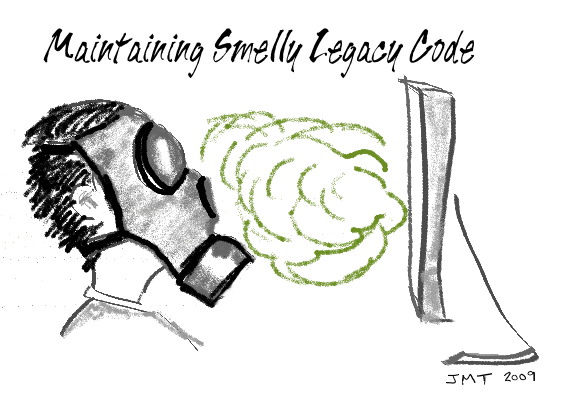
\includegraphics[scale=0.4]{img/SmellyLegacyCode}
\end{figure}
\end{frame}

\subsubsection{Stuck in the Past}
\begin{frame}\frametitle{Stuck in the Past}
  \begin{columns}
    \begin{column}{.5\linewidth}
      
\includegraphics[scale=0.3]{img/linkman}
       \end{column}
    \begin{column}{.5\linewidth}
      \begin{itemize}
      \item DOS compatibility mode
      \item Only works with MBRs
      \item CHS addressing
      \item Mainframe style UIs\newline
      \end{itemize}
    \end{column}
  \end{columns}
\end{frame}

\subsubsection{Everyone Looses}
\begin{frame}\frametitle{Everyone Looses}
    \begin{columns}
      \begin{column}{.5\linewidth}
        \begin{block}{Hackers loose}
          Adding new code and extending functionality is difficult, tedious and error prone.
        \end{block}
        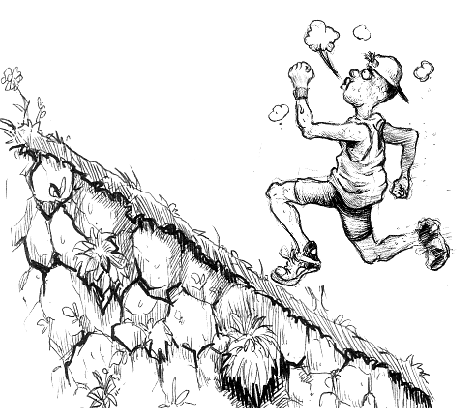
\includegraphics[scale=0.3]{img/running-uphill}
      \end{column}
      \begin{column}{.5\linewidth}
        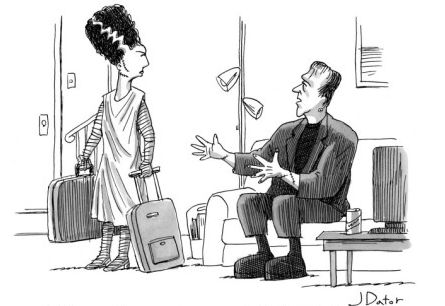
\includegraphics[scale=0.5]{img/leaving}
        \begin{block}{Users loose}
        Fdisk \textbf{cannot} compete with other partitioning tools and thus looses users. Hey, healthy competition is good for everyone!
        \end{block}
      \end{column}
    \end{columns}
  \end{frame}

\subsection{Fixing Fdisk}
\begin{frame}\frametitle{Short Term}
  Short term goals:
  \begin{itemize}
  \item Cleanup and refactor current, legacy, code
  \item Create an internal API that abstracts disklabel concepts and specifications
  \item Add GUID Partition Table (GPT) support
  \end{itemize}
\end{frame}

\begin{frame}\frametitle{Longer Term}
  Long term goals:
  \begin{itemize}
  \item Create an independent, libfdisk shared library.
  \item Rewrite cfdisk and sfdisk with new library.
  \end{itemize}
\end{frame}

% Copyright (C) 2012 Davidlohr Bueso <dave@gnu.org>

% API STUFF
\section{New Internal API}
\begin{frame}\frametitle{New Internal API}
  \begin{itemize}
  \item Create an abstraction level between fdisk-family tools and lower-level disklabel logic.
  \item Use a driver based model to deal with disklabels and handle \emph{events} through callbacks.
  \item The API can be seen as:
    \begin{enumerate}
    \item handle generic disk logic (like disk topology, sectors, MBR)
    \item gateway for disklabel specific demads (like probing or deleting a partition).
    \end{enumerate}
  \item Everything fdisk is capable of doing is goverened by a \textbf{fdisk context}.
  \item API users need not worry about internals.
  \end{itemize}
\end{frame}

\subsection{Architectural Overview}
\begin{frame}
  \center{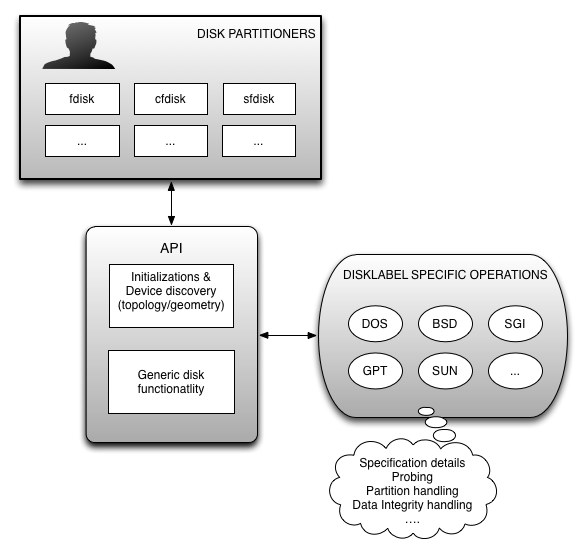
\includegraphics[scale=0.5]{img/fdisk-arch.png}}
\end{frame}

\subsection{API Benefits}
\begin{frame}\frametitle{API Benefits}
  \begin{itemize}
  \item Unifies concepts and specifications behind different partition formats; without hiding the details.
  \item Simplifies dealing with disklabel specifics.
  \item Makes the code easier to read and modify.
  \item Makes detecting existing bugs easier and reduces the probability of introducing new bugs.
  \item Once complete, the idea is to create a shared library - similar to what libparted is to GNU parted.
  \end{itemize}
\end{frame}

% Copyright (C) 2012 Davidlohr Bueso <dave@gnu.org>

% GPT STUFF
\section{GPT Support}
\begin{frame}\frametitle{What is GPT?}
  A standard developed by Intel in the late '90s for the layout of the partition table on a physical hard disk.\newline

  It overcomes major limitations of MBRs and today forms part of the \textbf{UEFI} standard.
\end{frame}

\subsection{Benefits of GPT}
\begin{frame}\frametitle{Benefits of GPT}
  So, what's the big deal about GPT?
  \begin{itemize}
  \item Forget extended or logical DOS-like partitions. GPT can handle at least 128 partitions.
  \item 64-bit sectors gives us $2^{64}$ available sectors, or 9.4 Zb partitions (with 512 bytes).
  \item 32-bit CRC checksums to ensure data integrity.
  \item Redundant data structures help protect against disk errors.
  \end{itemize}
\end{frame}

\subsection{Drawbacks of GPT}
\begin{frame}\frametitle{Drawbacks of GPT}
  \begin{columns}
    \begin{column}{.25\linewidth}
      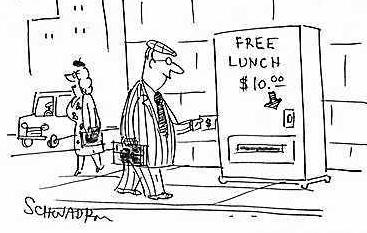
\includegraphics[scale=1.3]{img/freelunch}
    \end{column}
    \begin{column}{.7\linewidth}
      \begin{itemize}
      \item Compatibility
        \begin{itemize}
        \item OS
        \item Bootloaders
        \end{itemize}
      \item Non-standard schemes (Hybrid MBRs)
      \end{itemize}
    \end{column}
  \end{columns}
\end{frame}

\subsection{Fdisk and GPT}
\begin{frame}\frametitle{Fdisk \& GPT}
  \begin{itemize}
  \item Well known fact that fdisk didn't play well with GPT
    \begin{itemize}
      \item disklabel detection \emph{only}
      \item sends users to other tools (GNU parted)
      \item deals only with legacy DOS partitions.
    \end{itemize}
  \item Sept. 2012 we got full GPT support merged in mainline fdisk.
  \end{itemize}
\end{frame}

\subsection{Implementation Details}
\begin{frame}\frametitle{Some GPT Implementation Details}
  \begin{itemize}
  \item Deals with both legacy protective and hybrid MBRs.
  \item Updates checksums on the fly and not only when writing in-memory data to disk.
  \item Plays well with larger logical-sectors (4K)
  \item Generous support for GUID partition types.
  \end{itemize}
\end{frame}

% Copyright (C) 2012 Davidlohr Bueso <dave@gnu.org>

% THE ROAD AHEAD
\section{The Road Ahead}
\begin{frame}\frametitle{The Road Ahead}
  \begin{columns}
    \begin{column}{.5\linewidth}
      
\includegraphics[scale=0.4]{img/goals}
    \end{column}
    \begin{column}{.5\linewidth}
      \begin{itemize}
      \item Enhance UIs ($libreadline$ - gdb style)
      \item Support more disklabels (APM, AIX)
      \item General cleanups and refactoring
      \item Documentation
      \item tests, tests, tests
      \end{itemize}
    \end{column}
  \end{columns}      
\end{frame}


\begin{frame}\frametitle{Thank you}
  \center{ 
\includegraphics[scale=0.5]{img/thankyou} }
\end{frame}
\end{document}
